\chapter[RESULTADOS]{\textbf {RESULTADOS}}

\section[VISÃO GERAL]{VISÃO GERAL}
O estudo, objeto deste trabalho, foi realizado no período de quatro meses (Abril/2010 à
Agosto/2010) e gerou como resultado, um processo de trabalho para a execução de
projetos de integração entre RIS, PACS e mamógrafos digitais, além da submissão de um
artigo sobre o trabalho no CBEB XXII (XXII Congresso Brasileiro de Engenharia
Biomédica). O referido artigo encontra-se no Anexo ?? deste documento e o processo de
trabalho proposto é descrito a seguir.

O processo proposto é composto de fluxos de trabalho e modelos para a construção de
artefatos que documentam todas as atividades da integração. As atividades do processo
sugerido são organizadas em cinco etapas, quais sejam: (i) Levantamento de Requisitos;
(ii) Projeto de Integração; (iii) Execução da Integração; (iv) Avaliação da Integração e (v)
Treinamento. A Figura 22 ilustra essas etapas e indica que o trabalho contemplou os
conceitos das tecnologias RIS, PACS e de mamografia digital, além dos padrões DICOM e
IHE bastante conhecidos e aplicados na indústria médica.


\begin{figure}[ht]
 \centering
 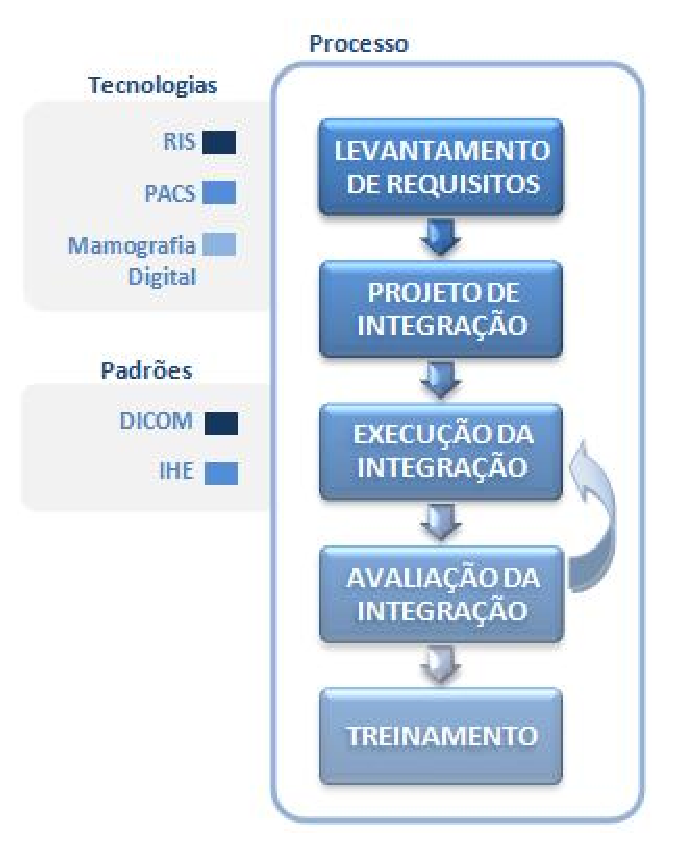
\includegraphics[width=6 cm]{figuras/fig2.eps}
 \caption{Fluxo principal do processo de integração de RIS, PACS e mamógrafos digitais.}
 \label{fig2}
\end{figure}


\section[LEVANTAMENTO DE REQUESITOS]{LEVANTAMENTO DE REQUESITOS}


A primeira etapa do processo de integração é o levantamento de requisitos. Essa etapa tem
como objetivos: (i) a compreensão das necessidades da unidade de saúde que pratica a
mamografia digital; (ii) a definição dos requisitos e limitações do projeto de integração e
(iii) o entendimento da infraestrutura tecnológica existente. A Figura \ref{fig2} mostra a
seqüência de atividades desta etapa e sugere alguns artefatos de trabalho.


